\documentclass[12pt]{../notes}

% Command for Questions
%\question{}

% Command for Notes
% \note{}

% Code to create a minipage where you can type in class notes. 
%%\begin{minipage}[l][2cm][c]{\textwidth}
%\begin{comment}

%\end{comment}
%%\end{minipage}


% Begin Document
%==============================================================================
\begin{document}
% Include the Title of the Handout
\ntitle{3.1 Alternate Variable Types and Interactions}

\question{Describe the difference between multicollinearity and interactions.}

\begin{minipage}[l][3cm][c]{\textwidth}
%\begin{comment}
\note{Multicollinearity only deals with relationships among the X variables and has NOTHING to do with Y. Interactions have EVERYTHING to do with Y and the way that $X_k$'s relationship with Y is influenced by the other X variables.}
%\end{comment}
\end{minipage}

\nspace
\question{Identify whether each of the following variables are qualitative or quantitative:}
\begin{itemize}
\item hours worked 
%\begin{comment} 
\note{quantitative} 
%\end{comment}
\item shirt color
%\begin{comment} 
\note{qualitative} 
%\end{comment}
\item a person's shoe size
%\begin{comment} 
\note{quantitative} 
%\end{comment}
\item systolic blood pressure
%\begin{comment} 
\note{quantitative} 
%\end{comment}
\item blood type
%\begin{comment} 
\note{qualitative} 
%\end{comment}
\item college major
%\begin{comment} 
\note{qualitative} 
%\end{comment}
\end{itemize}

\question{Ignoring the significance of the model coefficients and assuming that assumptions regarding residuals are satisfied, please write the estimated regression equation corresponding to the following SAS output (not that Y represents Oxygen Intake Rate).}

\begin{figure}[H]
\centering
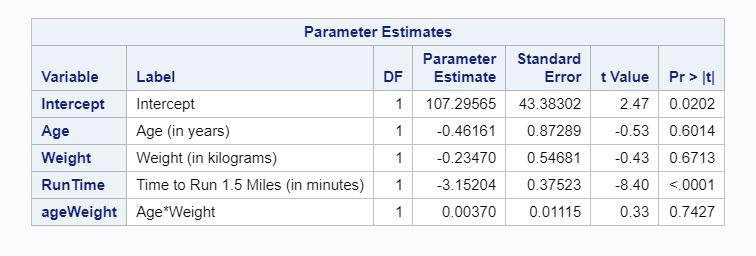
\includegraphics[width=\textwidth]{../figures/module3/age_weight_interaction_example.png}
\end{figure}

\begin{minipage}[l][2cm][c]{\textwidth}
%\begin{comment}
\note{$$\hat{Y} = 107.296 - 0.461*Age - 0.235*Weight - 3.152*RunTime + 0.004*Age*Weight$$}
%\end{comment}
\end{minipage}

\question{What is the expected change in the average of Y when a person ages by one year?}

\begin{minipage}[l][2cm][c]{\textwidth}
%\begin{comment}
\note{$$-0.461 + 0.004*Weight$$}
%\end{comment}
\end{minipage}

\question{Suppose you are trying to predict a person's happiness and you suspect that country of origin is a significant predictor of happiness. You take a sample of 100 people to test your hypothesis. In this scenario, what issue will you run into trying to use country of origin as a predictor variable?}

\begin{minipage}[l][2cm][c]{\textwidth}
%\begin{comment}
\note{We need $q-1$ dummy variables to represent $q$ countries. There are more than 100 countries in the world, so our model would require more degrees of freedom than is feasible with our sample size.}
%\end{comment}
\end{minipage}




% End the Document
%==============================================================================
\end{document}